\documentclass[12pt,a4paper]{report}
\usepackage[utf8]{inputenc}
\usepackage{graphicx}
\usepackage{url}
\usepackage{cite}
\usepackage{hyperref}
\usepackage{tikz}
\usetikzlibrary{shapes,arrows.meta,positioning,fit}
\usepackage{pgfplots}
\pgfplotsset{compat=1.18}
\hypersetup{
    colorlinks=true,
    linkcolor=blue,
    citecolor=blue,
    urlcolor=blue
}


\title{Log Anomaly Detection in Distributed Streaming Systems}
\author{Nikola Lichovski}
\date{}



\begin{document}

\maketitle
\tableofcontents

\chapter{Introduction}

In modern distributed systems, the continuous generation of application and infrastructure logs provides a critical foundation for monitoring, debugging, and performance optimization. However, the sheer volume, velocity, and diversity of log data make manual inspection or traditional rule-based monitoring inefficient and error-prone. As systems scale horizontally and operate across multiple services and nodes, automated methods for detecting abnormal behaviour in log streams become essential.

Log anomaly detection focuses on identifying unusual patterns or events in log data that may indicate failures, performance degradation, or security threats. When combined with streaming and distributed processing technologies such as Apache Kafka, these methods enable near real-time detection and response, ensuring higher system reliability and availability.

This project explores the design and evaluation of a distributed log \\anomaly detection pipeline. The system ingests log data through multiple parallel producers, processes it in real-time using a message broker, and applies anomaly detection algorithms on the consumer side. The results are stored in a database and visualized through a lightweight dashboard. 

The primary objectives are to:
\begin{itemize}
  \item Develop a distributed streaming architecture for log data processing and anomaly detection.
  \item Evaluate the performance of the system under different configurations of producers and consumers.
  \item Analyze the trade-offs between throughput, latency, and detection accuracy in a parallel environment.
\end{itemize}

The study aims to contribute to the broader understanding of scalable anomaly detection in parallel and distributed systems, emphasizing how distributed messaging frameworks can be leveraged to improve the responsiveness and reliability of monitoring pipelines.

The complete source code, experiment scripts, and configuration files used in this work are publicly available at:
\url{https://github.com/NikolaLichovski/distributed-log-ml-benchmark}.

\chapter{Related Work}

\section{Log Anomaly Detection in Modern Systems}  
In large-scale distributed systems, log data serves as the primary source of telemetry, capturing runtime events, service interactions, failures, and performance metrics. Logs are characterized by high volume, high velocity, and high variety, which makes manual monitoring or rule-based detection increasingly infeasible. Fu et al. \cite{Fu2009} demonstrated that statistical deviations in unstructured log data could reveal execution anomalies, establishing foundational techniques for automated log analysis. While effective in controlled settings, these approaches struggle with highly dynamic or evolving log streams.  

With the emergence of deep learning, sequence-based models such as LSTM have been applied to log streams, providing better capability to capture temporal dependencies and detect subtle anomalies \cite{Du2017}. Du et al. showed that modeling the sequential patterns of logs allows the detection of abnormal events that do not necessarily deviate in value but in order or context. Sun et al. \cite{Sun2021} extended these ideas to handle unlabeled and highly variable log data, highlighting the need for models that can adapt to evolving distributed system behaviors. These studies collectively underscore the shift from purely statistical to learning-based approaches in modern anomaly detection.

\section{Pipelines for Streaming and Distributed Log Processing}  
Real-time processing of logs in distributed systems requires robust streaming pipelines capable of parallelism, partitioning, and fault-tolerance. Mayer et al. \cite{Mayer2017} introduced StreamLearner, which demonstrates distributed incremental learning over event streams while maintaining state consistency across multiple nodes. Their work emphasizes the importance of designing pipelines that are both scalable and dynamically adaptable to varying workloads.  

Comparative studies on anomaly detection algorithms in streaming environments \cite{Hasani2020} reveal that detection accuracy, latency, and computational efficiency vary significantly depending on the pipeline design. This shows that the choice of framework and algorithm cannot be separated from architectural considerations. Wu et al. \cite{Wu2021} surveyed log analysis techniques and concluded that integrating adaptive streaming frameworks with anomaly detection pipelines is essential for maintaining reliability under high-throughput conditions. Together, these works highlight that an effective anomaly detection system depends not only on the detection algorithm but also on a well-designed, fault-tolerant streaming pipeline.

\section{Anomaly Detection Techniques for Log Data}  
Methodologically, log anomaly detection spans statistical techniques, classical machine learning, and deep learning. Statistical methods often rely on outlier detection or dimensionality reduction to identify unusual events \cite{Fu2009}. These methods are computationally efficient but limited in capturing complex patterns. Deep learning approaches, particularly sequence models such as LSTM, have proven effective in modeling temporal dependencies and contextual anomalies \cite{Du2017, Sun2021}. They can detect anomalous sequences that may appear normal when considering individual log entries in isolation.  

Multi-source techniques, as presented by Bogatinovski et al. \cite{Bogatinovski2021}, extend anomaly detection by combining heterogeneous log streams from distributed systems. This approach improves robustness against missing or inconsistent data and can capture correlations across multiple services or nodes. 

\section{Log Anomaly Detection in Distributed / Parallel Settings}  
Distributed and parallel systems introduce additional challenges: logs may arrive out-of-order, services may produce heterogeneous formats, and system scaling (multiple producers and consumers) can impact detection latency and throughput. Han et al. \cite{Han2023} and Himler et al. \cite{Himler2024} demonstrated that deep learning-based distributed anomaly detection benefits from explicitly modeling the distributed context, leading to improved accuracy and responsiveness.  

Benchmark studies of streaming pipelines \cite{Patel2024} reveal that parallelism and partitioning strategies strongly influence system performance metrics, such as throughput and end-to-end latency. Edge-oriented frameworks such as IDForest \cite{IDForest2022} further illustrate that lightweight, incremental models can detect anomalies in real-time with minimal resource overhead. These findings emphasize that both the detection algorithm and the distributed system design contribute critically to effective log anomaly detection.

\section{Positioning of This Work}

Despite extensive research on log anomaly detection algorithms and streaming system architectures, few studies systematically evaluate the \textbf{interaction between system configuration and detection performance} in distributed settings. Most prior work focuses on either algorithmic improvements (accuracy, model architecture) or system design (throughput, fault tolerance), treating these as independent concerns.

However, as highlighted by Patel et al. \cite{Patel2024}, performance benchmarks often neglect the impact of distributed system parameters—such as partition count, consumer group size, and producer parallelism—on both computational efficiency and detection reliability. Himler et al. \cite{Himler2024} note that distributed anomaly detection introduces challenges of model consistency and coordination overhead, but provide limited quantitative analysis of these effects under varying configurations.

This work addresses these gaps through controlled experimentation that systematically varies three architectural parameters (producer count, consumer count, partition count) and measures their combined impact on four performance dimensions (throughput, latency, consumer lag, anomaly detection rate). Specifically, this study provides:

\begin{itemize}
    \item \textbf{Empirical measurement} of throughput scaling characteristics under parallel log ingestion
    \item \textbf{Quantitative analysis} of consumer group coordination overhead and its impact on lag accumulation
    \item \textbf{Critical evaluation} of distributed anomaly detection consistency when models operate independently per consumer
    \item \textbf{Practical guidance} on configuration selection for balancing performance and detection reliability
\end{itemize}

By treating the system as a unified experimental platform rather than separating algorithm from architecture, this work demonstrates that configuration choices significantly influence not only processing performance but also the reliability and consistency of anomaly detection results. These findings are directly relevant to practitioners deploying log analysis pipelines in production distributed systems.

The present work addresses this gap by implementing a distributed streaming pipeline and measuring performance across multiple dimensions. By adjusting producer and consumer counts and observing the resulting effects on latency, throughput, and detection accuracy, this study provides practical insights into the trade-offs inherent in distributed log anomaly detection. Furthermore, it demonstrates how a modular pipeline can be configured to balance system efficiency with detection reliability, offering guidance for both researchers and practitioners designing similar systems.


\chapter{Solution Architecture}

\section{Overview}

The goal of this architecture is to design a distributed log anomaly detection pipeline capable of ingesting streaming log data, processing it in real time, identifying anomalous behaviour, and storing both detections and performance metrics for later analysis. The system is planned to be modular and easy to reconfigure, since part of the work involves experimenting with different numbers of producers, consumers, and Kafka partitions. For anomaly detection, the initial approach will rely on an Isolation Forest model, mainly because it works well with high-volume data streams and does not require labelled examples \cite{IDForest2022, Bogatinovski2021}.

\section{High-level workflow}

The pipeline consists of several components that interact through well-defined interfaces: log producers, a Kafka broker, consumer services that carry out feature extraction and anomaly scoring, a relational database for persistence, and a dashboard for real-time monitoring.  
Figure~\ref{fig:architecture} summarizes the planned data flow.

\begin{enumerate}
    \item \textbf{Producers} generate or relay structured JSON logs at a configurable rate. Multiple instances can be started to simulate higher input load.
    \item \textbf{Kafka} acts as the ingestion layer. Producers write logs to partitioned topics, allowing parallel processing \cite{Mayer2017}.
    \item \textbf{Consumers} subscribe as a consumer group. Each instance extracts simple features from incoming logs and assigns anomaly scores using Isolation Forest.
    \item \textbf{PostgreSQL} stores both the processed logs and anomaly scores. An additional table is planned for recording run-level performance metrics.
    \item \textbf{Dashboard (Streamlit)} visualizes throughput, lag, anomaly counts, and other collected metrics.
    \item \textbf{Orchestration} is handled with Docker Compose, which makes it possible to scale producers and consumers for controlled experiments.
\end{enumerate}

\begin{figure}[htbp]
\centering
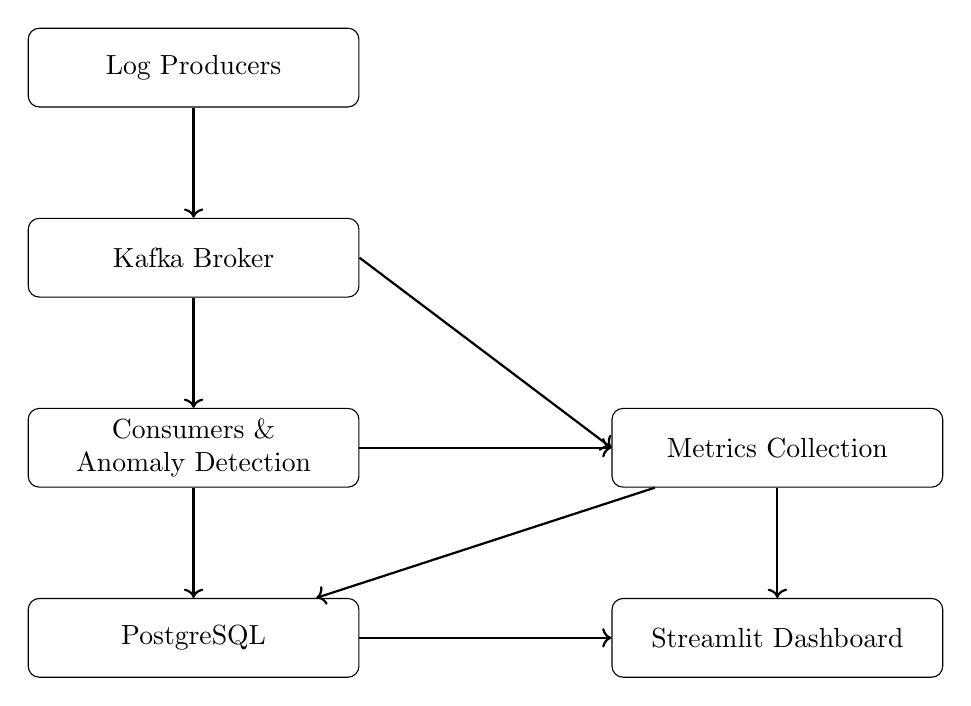
\begin{tikzpicture}[
    comp/.style={draw, rounded corners, fill=white, minimum width=4.2cm, minimum height=1cm, align=center},
    arrow/.style={->, thick},
    node distance=1.4cm
]

% main pipeline
\node[comp] (producers) {Log Producers};
\node[comp, below=of producers] (kafka) {Kafka Broker};
\node[comp, below=of kafka] (consumers) {Consumers \&\\ Anomaly Detection};
\node[comp, below=of consumers] (database) {PostgreSQL};

% side components (placed tighter, no overflow)
\node[comp, right=3.2cm of consumers] (metrics) {Metrics Collection};
\node[comp, below=of metrics] (dashboard) {Streamlit Dashboard};

% arrows (pipeline)
\draw[arrow] (producers) -- (kafka);
\draw[arrow] (kafka) -- (consumers);
\draw[arrow] (consumers) -- (database);

% arrows (metrics + dashboard)
\draw[arrow] (kafka.east) -- (metrics.west);
\draw[arrow] (consumers.east) -- (metrics.west);
\draw[arrow] (metrics) -- (database);
\draw[arrow] (metrics) -- (dashboard);
\draw[arrow] (database) -- (dashboard);

\end{tikzpicture}
\caption{Planned high-level architecture of the log anomaly detection pipeline.}
\label{fig:architecture}
\end{figure}

\section{Data Flow}

Alongside the architectural overview, the data-flow diagram ~\ref{fig:dataflow} presents the planned path that each log entry will take through the platform. The process will begin with log creation, continue with structured ingestion into Kafka, then pass through the machine-learning consumer for feature extraction and anomaly scoring. The results will then be inserted into PostgreSQL and displayed on the dashboard. By laying out this future workflow, the diagram shows how the system is expected to operate in practice.

\begin{figure}[htbp]
\centering
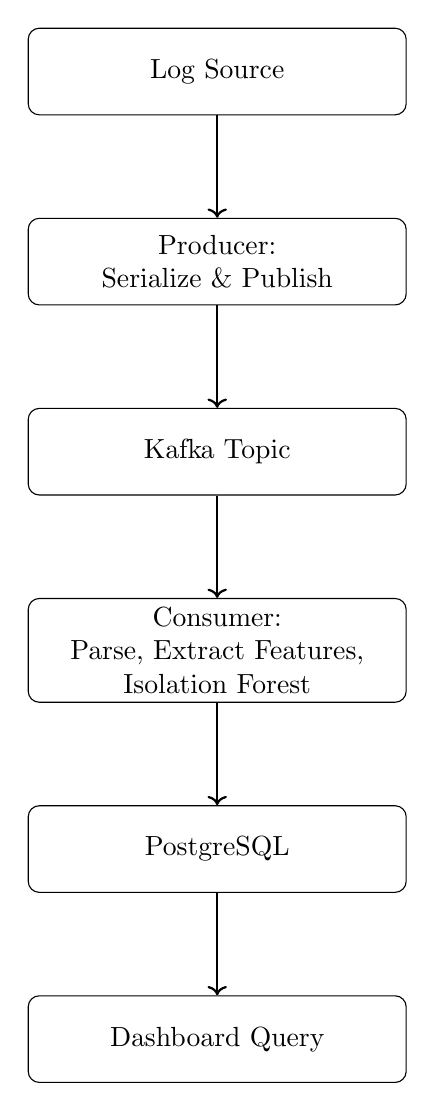
\begin{tikzpicture}[
    comp/.style={draw, rounded corners, fill=white, minimum width=4.8cm, minimum height=1.1cm, align=center},
    arrow/.style={->, thick},
    node distance=1.3cm
]

\node[comp] (src) {Log Source};
\node[comp, below=of src] (prod) {Producer:\\Serialize \& Publish};
\node[comp, below=of prod] (kfk) {Kafka Topic};
\node[comp, below=of kfk] (cons) {Consumer:\\Parse, Extract Features,\\Isolation Forest};
\node[comp, below=of cons] (db) {PostgreSQL};
\node[comp, below=of db] (dash) {Dashboard Query};

\draw[arrow] (src) -- (prod);
\draw[arrow] (prod) -- (kfk);
\draw[arrow] (kfk) -- (cons);
\draw[arrow] (cons) -- (db);
\draw[arrow] (db) -- (dash);

\end{tikzpicture}
\caption{Data-flow diagram of the planned anomaly detection pipeline.}
\label{fig:dataflow}
\end{figure}

\section{Component Implementation}

\subsection{Log Producers}

Producers are implemented as containerized Python processes using the \texttt{confluent-kafka} library. Each producer instance generates synthetic JSON log entries at a configurable rate (default: 1.0 messages per second) and publishes them to the Kafka topic. Log entries contain four fields: timestamp (ISO 8601 format), service identifier (chosen from a predefined set of five microservices), log level (INFO, WARN, or ERROR with weighted probability distribution), and message text.

To support systematic experimentation, each producer instance:
\begin{itemize}
    \item Accepts environment variables for experiment ID and target message rate
    \item Records message send timestamps for latency calculation
    \item Implements delivery callbacks to confirm successful broker acknowledgment
    \item Publishes metrics (throughput, send latency) to PostgreSQL via a shared metrics collection library
\end{itemize}

Multiple producer instances operate independently and do not coordinate with each other. Each produces messages with unique keys, enabling Kafka's partition assignment logic to distribute load across available partitions.

\subsection{Apache Kafka and Partitioning Strategy}

Kafka serves as the distributed message buffer between producers and consumers. The system uses a single topic with a configurable number of partitions (1, 3, or 6 in the experiments). Partitions enable parallel consumption: each partition is assigned to exactly one consumer within a consumer group, allowing multiple consumers to process different subsets of the log stream concurrently.

Key configuration parameters include:
\begin{itemize}
    \item \textbf{Replication factor:} Set to 1 (single broker, suitable for experimental environment)
    \item \textbf{Retention policy:} Messages retained for the duration of experiments
    \item \textbf{Auto-creation:} Disabled; topics created programmatically with specified partition count
\end{itemize}

Partition assignment follows Kafka's default range-based strategy. For example, with 3 partitions and 2 consumers, one consumer receives partitions 0 and 1, while the other receives partition 2. This creates potential load imbalance, which is reflected in the experimental results.

\subsection{Consumer Group and Parallel Processing}

Consumers are implemented as containerized Python processes that subscribe to the log topic as members of a shared consumer group (\texttt{ml-consumer-group}). Kafka's consumer group protocol ensures that each partition is assigned to exactly one consumer instance, preventing duplicate processing while enabling parallelism.

Each consumer implements the following processing pipeline:

\begin{enumerate}
    \item \textbf{Message polling:} Fetch batches of messages from assigned partitions (poll timeout: 1 second)
    \item \textbf{Deserialization:} Parse JSON log structure and validate required fields
    \item \textbf{Feature extraction:} Extract seven features for anomaly detection:
    \begin{itemize}
        \item Service identifier (label-encoded to integer)
        \item Log level (label-encoded: INFO=0, WARN=1, ERROR=2)
        \item Message length (character count)
        \item Error keyword presence (binary: 0 or 1)
        \item Warning keyword presence (binary: 0 or 1)
        \item Hour of day (0-23)
        \item Minute of hour (0-59)
    \end{itemize}
    \item \textbf{Anomaly scoring:} Apply Isolation Forest model to feature vector
    \item \textbf{Database insertion:} Store log entry and anomaly score in PostgreSQL
    \item \textbf{Offset commit:} Acknowledge successful processing to Kafka
    \item \textbf{Metrics recording:} Log processing latency and current partition lag
\end{enumerate}

\textbf{Critical implementation detail:} Each consumer maintains an \textit{independent} Isolation Forest model, trained on its own partition's historical data (last 1000 messages, minimum 10 for training). Models are persisted to a Docker volume to survive consumer restarts. This design choice, while simplifying implementation, introduces model divergence issues documented in the Results section.

\subsection{Isolation Forest Anomaly Detection}

The Isolation Forest algorithm \cite{IDForest2022} detects anomalies by measuring how easily a data point can be isolated in randomly constructed decision trees. Anomalies, being rare and different, require fewer splits to isolate compared to normal points.

Model parameters:
\begin{itemize}
    \item \textbf{Contamination:} 0.1 (expects 10\% of data to be anomalous)
    \item \textbf{Number of estimators:} 100 trees
    \item \textbf{Random state:} Fixed at 42 for reproducibility
\end{itemize}

The model triggers retraining every 20 messages if not yet trained, using the most recent 1000 historical logs from the database. For each incoming log, the model returns:
\begin{itemize}
    \item \textbf{Binary prediction:} Anomaly (−1) or normal (+1)
    \item \textbf{Anomaly score:} Decision function value, normalized to [0, 1] range
\end{itemize}

\subsection{Performance Metrics Collection}

A shared Python library (\texttt{metrics\_collector.py}) provides thread-safe metrics collection with batched database writes. Both producers and consumers instantiate a \texttt{MetricsCollector} object configured with:
\begin{itemize}
    \item Experiment ID (for grouping related measurements)
    \item Component type and instance ID
    \item Batch size (50 metrics) and flush interval (10 seconds)
\end{itemize}

Producers record:
\begin{itemize}
    \item Message send latency (time from creation to broker acknowledgment)
    \item Per-producer throughput (messages per second, windowed)
\end{itemize}

Consumers record:
\begin{itemize}
    \item End-to-end processing latency (message receipt to database commit)
    \item Per-consumer throughput (messages processed per second)
    \item Consumer lag per partition (current offset vs. log-end offset)
\end{itemize}

Metrics are buffered in memory and inserted into PostgreSQL in batches to minimize database overhead. A background thread performs periodic flushes every 10 seconds or when the buffer reaches 50 entries.

\subsection{Database Schema}

PostgreSQL stores five types of data:

\begin{enumerate}
    \item \textbf{Logs table:} Raw log entries (timestamp, service, level, message)
    \item \textbf{Anomalies table:} Detection results (foreign key to logs, binary flag, score)
    \item \textbf{Experiments table:} Metadata for each run (producers, consumers, partitions, start/end time, status)
    \item \textbf{Performance\_metrics table:} Time-series measurements (experiment ID, component type/ID, metric name, value, timestamp)
    \item \textbf{Consumer\_lag table:} Partition-level lag tracking (experiment ID, consumer ID, partition, offsets, timestamp)
\end{enumerate}

Indexes are created on frequently queried columns (timestamps, experiment ID, component IDs) and composite indexes support common query patterns (e.g., filtering metrics by experiment and component type).

\subsection{Orchestration and Experiment Management}

Docker Compose manages all services (ZooKeeper, Kafka, PostgreSQL, producers, consumers, dashboard) and supports dynamic scaling through environment variables:

\begin{itemize}
    \item \texttt{EXPERIMENT\_ID}: Unique identifier for grouping metrics
    \item \texttt{KAFKA\_NUM\_PARTITIONS}: Partition count for topic creation
    \item \texttt{LOG\_RATE}: Messages per second per producer
\end{itemize}

The \texttt{run\_experiment.sh} shell script automates experimental runs:
\begin{enumerate}
    \item Create experiment record in database with configuration parameters
    \item Set environment variables (experiment ID, partition count, log rate)
    \item Scale producer and consumer services using \texttt{docker-compose up --scale}
    \item Monitor experiment for specified duration
    \item Update experiment status to "completed" in database
    \item Query and display summary statistics (total logs, throughput, latency, lag)
\end{enumerate}

This automation enables reproducible experiments and systematic performance comparison across configurations.

\section{Scalability and Planned Extensions}

The architecture is designed to scale horizontally by simply adding more producers or consumers. Kafka’s partitioning provides a natural parallelism model, and the database schema will support tracking performance across different runs.  
Future work may include exploring alternative anomaly detection approaches that incorporate temporal patterns or sequence modelling \cite{Du2017, Sun2021}, but the first version will focus on Isolation Forest and feature-based detection.


\chapter{Results}

This chapter presents and analyzes the experimental results obtained from the distributed
log anomaly detection system. The \textbf{parallel and distributed component of the system
consists of three cooperating layers}: (1) multiple concurrent Kafka producer processes that
independently publish log events to a partitioned topic, (2) a Kafka broker that distributes
messages across partitions, enabling parallel consumption, and (3) a consumer group of
independent worker processes that each consume an assigned subset of partitions and run
Isolation Forest inference in parallel. Orchestration of all components is handled through
Docker Compose, which enables scaling each layer independently without code changes.

The experiments evaluate how the \textbf{degree of parallelism}---controlled by varying the
number of producers, consumers, and Kafka partitions---affects throughput, latency, consumer
lag, and anomaly detection behavior. The single-producer, single-consumer, single-partition
configuration serves as the \textbf{sequential reference
point}: all log generation, message brokering, and anomaly detection occur without any
parallelism. Every subsequent configuration introduces parallelism at one or more layers,
allowing direct measurement of the performance gains and trade-offs introduced by the
distributed implementation.

Each experiment ran for 10 minutes with identical log generation patterns and Isolation
Forest model parameters (contamination=0.1, n\_estimators=100).

\textbf{Important note:} All experiments used the same log generation rate of 1.0 messages
per second per producer. Therefore, differences in total processed logs primarily reflect
the number of active producers rather than differences in system capacity or processing speed.

% ---------------------------------------------------------------
\section{Overview of Experiments}

Table~\ref{tab:all-experiments} presents results from ten configurations designed to isolate
the effects of scaling producers, consumers, and Kafka partitions. The configurations
progress from fully sequential (1P-1C-1Part) to increasingly parallel, culminating in the
stress-test configuration (4P-4C-6Part), which maximizes parallelism at every layer of the
pipeline.

% [TABLE 4.1 UNCHANGED]
\begin{table}[htbp]
\centering
\caption{Summary of experimental results across all configurations}
\label{tab:all-experiments}
\small
\begin{tabular}{@{}lcccccccc@{}}
\hline
\textbf{Experiment} & \textbf{P} & \textbf{C} & \textbf{Part.} & \textbf{Logs} &
\textbf{Anom.} & \textbf{Thr.} & \textbf{Lat. (ms)} & \textbf{Lag} \\
\hline
baseline-1p-1c-1part & 1 & 1 & 1 & 593  & 48  & 0.99 & 506.80 & 1001 \\
baseline-1p-1c-3part & 1 & 1 & 3 & 593  & 70  & 0.99 & 506.80 & 1001 \\
scale-producers-2p   & 2 & 1 & 3 & 1188 & 233 & 1.42 & 595.52 & 1244 \\
scale-producers-3p   & 3 & 1 & 3 & 1816 & 361 & 2.02 & 493.33 & 1730 \\
scale-consumers-2c   & 1 & 2 & 3 & 639  & 130 & 1.00 & 506.61 & 2466 \\
scale-consumers-3c   & 1 & 3 & 3 & 619  & 54  & 1.00 & 506.61 & 2712 \\
balanced-2p-2c       & 2 & 2 & 3 & 1228 & 157 & 1.52 & 486.69 & 2961 \\
balanced-3p-3c       & 3 & 3 & 3 & 1851 & 375 & 2.01 & 493.23 & 3459 \\
high-partitions      & 2 & 2 & 6 & 1210 & 246 & 1.51 & 486.84 & 1009 \\
stress-test-4p-4c    & 4 & 4 & 6 & 2460 & 512 & 2.48 & 506.48 & 1260 \\
\hline
\multicolumn{9}{p{\linewidth}}{\footnotesize
Thr.\ = Throughput (msg/s), Lat.\ = Latency,
Lag = Max Lag (messages), P = Producers,
C = Consumers, Part.\ = Partitions}
\end{tabular}
\end{table}

% ---------------------------------------------------------------
\section{Baseline Performance and Partition Effects}

The baseline configuration (1 producer, 1 consumer, 1 partition) represents the
\textbf{fully sequential execution path} of the pipeline: a single process generates logs,
a single Kafka partition serializes all messages, and a single consumer performs anomaly
detection without any concurrency. This configuration establishes the reference performance
values against which all parallel configurations are compared: 593 processed logs, 0.99
msg/s throughput, 506.8ms average latency, and 1001 messages maximum lag. The system
detected 48 anomalies (8.1\% of total logs).

Increasing partitions from 1 to 3 while maintaining single producer and consumer
\textbf{introduces broker-level parallelism without adding consumer parallelism}, since a
single consumer still handles all partitions alone. Consequently, no throughput or latency
improvement is observed, confirming that partition count alone does not improve performance
unless matched with additional consumers. However, the anomaly count increased from 48 to
70 (11.8\% of logs). This 46\% increase in detected anomalies warrants investigation, as it
suggests partition-based message distribution may affect the Isolation Forest's ability to
identify outliers. Possible explanations include:

\begin{itemize}
    \item \textbf{Partition key effects:} Different partition assignment may alter the local
    distribution of log features within consumer batches
    \item \textbf{Training data composition:} The model trains on the last 1000 logs;
    partition distribution could affect which logs constitute the training set
    \item \textbf{Temporal ordering changes:} Multi-partition consumption may process logs
    in different order, affecting feature extraction
\end{itemize}

This observation highlights that \textbf{Kafka partitioning configuration can influence
anomaly detection behavior beyond performance considerations}, an important finding for
production deployments.

% [TABLE 4.2 UNCHANGED]
\begin{table}[htbp]
\centering
\small
\caption{Effect of partition count on baseline configuration}
\label{tab:partition-effect}
\begin{tabular}{@{}lccccc@{}}
\hline
\textbf{Partitions} & \textbf{Throughput} & \textbf{Latency (ms)} & \textbf{Max Lag} &
\textbf{Anomalies} & \textbf{Rate} \\
\hline
1 & 0.99 & 506.80 & 1001 & 48 & 8.1\% \\
3 & 0.99 & 506.80 & 1001 & 70 & 11.8\% \\
\hline
\multicolumn{6}{@{}l@{}}{\footnotesize \textit{Note: 46\% increase in anomaly detection
requires further investigation}}
\end{tabular}
\end{table}

% ---------------------------------------------------------------
\section{Producer Scaling Analysis}

% [TABLE 4.3 UNCHANGED]
\begin{table}[htbp]
\centering
\small
\caption{Producer scaling with single consumer (3 partitions)}
\label{tab:producer-scaling}
\begin{tabular}{@{}lccccc@{}}
\hline
\textbf{Producers} & \textbf{Logs} & \textbf{Throughput} & \textbf{Latency (ms)} &
\textbf{Max Lag} & \textbf{Anom. Rate} \\
\hline
1 & 593  & 0.99 & 506.80 & 1001 & 11.8\% \\
2 & 1188 & 1.42 & 595.52 & 1244 & 19.6\% \\
3 & 1816 & 2.02 & 493.33 & 1730 & 19.9\% \\
\hline
\end{tabular}
\end{table}


These experiments measure the effect of \textbf{scaling parallelism at the ingestion layer}
while keeping consumer capacity fixed at one instance. Each additional producer is an
independent process running concurrently, publishing to the shared Kafka topic without
coordination with other producers. Table~\ref{tab:producer-scaling} shows the results.

Producer scaling demonstrates near-linear throughput scaling: doubling producers increases
throughput by 43\%, and tripling increases it by 104\%. This confirms that each producer
operates independently at approximately 1.0 msg/s, and that \textbf{Kafka successfully
absorbs concurrent writes from multiple producers without introducing write contention}.
The near-linear scaling validates the distributed ingestion design, where producers are
deliberately decoupled from one another and from the consumer layer.

\textbf{Critical observation:} The single consumer successfully processes input from
multiple producers without becoming saturated. Maximum lag grows (1001 $\rightarrow$ 1244
$\rightarrow$ 1730 messages), but remains bounded and proportional to total input rate.
This growing lag demonstrates that \textbf{the consumer is the bottleneck when ingestion
parallelism is increased without matching processing parallelism} --- a direct consequence
of the asymmetric scaling. The latency spike at 2 producers (595.52ms vs 506.80ms baseline)
followed by recovery at 3 producers (493.33ms) suggests transient consumer group
rebalancing overhead during partition reassignment.

\textbf{Anomaly detection consistency:} The anomaly rate stabilizes at approximately
19.6--19.9\% for multi-producer configurations, significantly higher than single-producer
scenarios (8.1--11.8\%). This increase is likely attributable to the Isolation Forest model
encountering greater diversity in log patterns when messages from multiple producers are
interleaved, leading to more outlier classifications during the initial training phase.

% ---------------------------------------------------------------
\section{Consumer Scaling Analysis}

% [TABLE 4.4 UNCHANGED]
\begin{table}[htbp]
\centering
\small
\caption{Consumer scaling with single producer (3 partitions)}
\label{tab:consumer-scaling}
\begin{tabular}{@{}lccccc@{}}
\hline
\textbf{Consumers} & \textbf{Logs} & \textbf{Throughput} & \textbf{Latency (ms)} &
\textbf{Max Lag} & \textbf{Anom. Rate} \\
\hline
1 & 593 & 0.99 & 506.80 & 1001 & 11.8\% \\
2 & 639 & 1.00 & 506.61 & 2466 & 20.3\% \\
3 & 619 & 1.00 & 506.61 & 2712 & 8.7\%  \\
\hline
\end{tabular}
\end{table}

These experiments measure the effect of \textbf{scaling parallelism at the processing
layer} while keeping ingestion fixed. In a Kafka consumer group, each consumer instance
is assigned a disjoint subset of partitions and processes them independently and
concurrently --- this is the primary mechanism for parallel anomaly detection in the
system. With a single producer generating 1.0 msg/s and 3 partitions, the input rate is
low enough that even one consumer keeps up. Adding consumers therefore does not increase
throughput (which remains at 1.00 msg/s), because the \textbf{bottleneck shifts to the
producer rather than the consumer}.

\textbf{Anomalous result:} Adding consumers \textit{increases} maximum lag from 1001 to
2466 (2 consumers) and 2712 (3 consumers). Rather than improving processing, adding more
parallel consumers \textbf{introduces distributed coordination overhead} through Kafka's
consumer group protocol. When a new consumer joins the group, Kafka triggers a partition
rebalancing event that temporarily halts all consumption while partitions are reassigned.
Under a low-throughput producer, the messages that accumulate during this stall are not
recovered quickly, causing measured lag to remain elevated. Potential causes include:

\begin{itemize}
    \item \textbf{Partition rebalancing overhead:} Kafka consumer group rebalancing causes
    temporary processing stalls during which lag accumulates
    \item \textbf{Offset commit contention:} Multiple consumers committing offsets to the
    same group coordinator may introduce serialization delays
    \item \textbf{Training data conflicts:} Each consumer maintains its own Isolation
    Forest model, trained on its partition's data; model divergence could affect processing
    efficiency
\end{itemize}

\textbf{Anomaly detection instability:} The dramatic drop in anomalies from 130 (2
consumers, 20.3\%) to 54 (3 consumers, 8.7\%) is a direct consequence of the
\textbf{distributed model architecture}. Because each consumer instance trains an
independent Isolation Forest on only the partition data it processes, the models diverge:
they learn from different log subsets and establish different decision boundaries. This
leads to:

\begin{enumerate}
    \item Different training data per consumer
    \item Divergent learned thresholds for anomaly classification
    \item Inconsistent anomaly detection across partitions
\end{enumerate}

This finding reveals a \textbf{critical limitation of the distributed design}: parallelizing
the anomaly detection layer without a model synchronization mechanism produces unreliable
and non-reproducible detection results.

% ---------------------------------------------------------------
\section{Balanced Scaling and System Optimization}

% [TABLE 4.5 UNCHANGED]
\begin{table}[htbp]
\centering
\caption{Balanced producer-consumer scaling (3 partitions, then 6)}
\label{tab:balanced}
\begin{tabular}{@{}lcccccc@{}}
\hline
\textbf{Config} & \textbf{P} & \textbf{C} & \textbf{Part.} & \textbf{Throughput} &
\textbf{Max Lag} & \textbf{Anom. Rate} \\
\hline
2P-2C     & 2 & 2 & 3 & 1.52 & 2961 & 12.8\% \\
3P-3C     & 3 & 3 & 3 & 2.01 & 3459 & 20.3\% \\
High-Part & 2 & 2 & 6 & 1.51 & 1009 & 20.3\% \\
Stress    & 4 & 4 & 6 & 2.48 & 1260 & 20.8\% \\
\hline
\end{tabular}
\end{table}

These configurations evaluate \textbf{full-pipeline parallelism}, where ingestion,
brokering, and processing layers all scale simultaneously. Balanced scaling maintains
throughput linearity (1.52 $\rightarrow$ 2.01 $\rightarrow$ 2.48 msg/s), confirming that
\textbf{the distributed pipeline scales proportionally when all layers are expanded
together}. However, when partition count (3) is insufficient relative to the number of
producers and consumers (3P-3C), lag grows to 3459 messages, indicating that Kafka's
parallelism ceiling has been reached.

The high-partition configuration (2P-2C-6Part) demonstrates that \textbf{increasing
broker-level parallelism dramatically reduces lag} (1009 vs 2961 messages for the equivalent
3-partition configuration), confirming that partition count is the primary constraint on
effective distributed throughput in this architecture.

\textbf{Key insight:} The stress test (4P-4C-6Part) achieves best overall performance:
highest throughput (2.48 msg/s), moderate lag (1260), and stable latency (506.48ms).
This configuration represents the most effective use of parallelism across all three layers
simultaneously. Comparing it to 3P-3C-3Part reveals that adequate partition count (6 vs 3)
prevents lag accumulation even under higher total load, demonstrating that
\textbf{partition count must scale with consumer count to unlock full distributed
processing capacity}.

% ---------------------------------------------------------------
\section{Latency Analysis and System Bottlenecks}

Figure~\ref{fig:latency-comparison} visualizes end-to-end latency across all ten
configurations. End-to-end latency here measures the time between a log message being
published to Kafka and the completion of its anomaly detection and database storage by a
consumer. It therefore captures the \textbf{total cost of the distributed processing
pipeline}, including network transit through Kafka, consumer group coordination, feature
extraction, and Isolation Forest inference.

% [FIGURE UNCHANGED]
\begin{figure}[htbp]
\centering
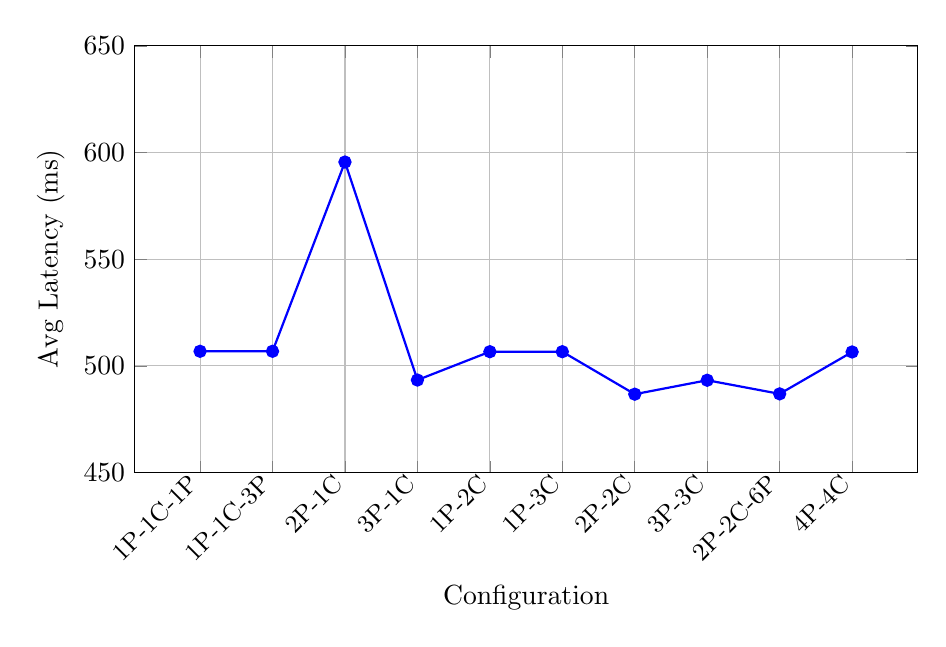
\begin{tikzpicture}
\begin{axis}[
    width=0.95\textwidth,
    height=7cm,
    xlabel={Configuration},
    ylabel={Avg Latency (ms)},
    symbolic x coords={1P-1C-1P, 1P-1C-3P, 2P-1C, 3P-1C, 1P-2C, 1P-3C,
                       2P-2C, 3P-3C, 2P-2C-6P, 4P-4C},
    xtick=data,
    x tick label style={rotate=45,anchor=east,font=\small},
    ymin=450, ymax=650,
    grid=major,
    every axis plot/.append style={thick}
]
\addplot[mark=*,blue] coordinates {
    (1P-1C-1P,506.80)
    (1P-1C-3P,506.80)
    (2P-1C,595.52)
    (3P-1C,493.33)
    (1P-2C,506.61)
    (1P-3C,506.61)
    (2P-2C,486.69)
    (3P-3C,493.23)
    (2P-2C-6P,486.84)
    (4P-4C,506.48)
};
\end{axis}
\end{tikzpicture}
\caption{Average end-to-end latency across all configurations. Latency remains stable
across sequential and parallel configurations, indicating that distributed overhead does
not measurably increase per-message processing time.}
\label{fig:latency-comparison}
\end{figure}

The latency clustering around 500ms ($\pm$20ms across all configurations) is a significant
result: it demonstrates that \textbf{introducing parallelism at any layer of the distributed
pipeline does not increase per-message processing latency}. In other words, scaling from
the sequential baseline (1P-1C-1Part) to the fully parallel stress test (4P-4C-6Part)
incurs no latency penalty. The dominant cost is the fixed Isolation Forest inference and
database write overhead, not distributed coordination. The 595.52ms spike at 2P-1C is the
only notable exception and is attributable to a transient consumer group rebalancing event
rather than a structural scaling limitation.

% ---------------------------------------------------------------
\section{Critical Findings and Limitations}

\subsection{Performance Scalability}

\textbf{Positive results --- where parallelism works:}
\begin{itemize}
    \item \textbf{Producer-layer parallelism scales linearly:} Each additional producer
    contributes approximately 1.0 msg/s of throughput, and Kafka absorbs concurrent writes
    without contention
    \item \textbf{Latency is unaffected by distribution:} End-to-end latency remains stable
    (~490--510ms) across all configurations, confirming negligible distributed overhead
    \item \textbf{Partition count governs effective parallelism:} Increasing partitions
    directly reduces lag accumulation and enables higher consumer concurrency
\end{itemize}

\textbf{Identified bottlenecks --- where parallelism underperforms:}
\begin{itemize}
    \item \textbf{Consumer-layer parallelism is only effective when matched with sufficient
    partitions:} Consumer group coordination overhead increases lag when consumer count
    exceeds partition count
    \item \textbf{Asymmetric scaling degrades performance:} Scaling producers without
    scaling consumers causes unbounded lag growth; scaling consumers without scaling
    producers yields no improvement
    \item \textbf{Producer rate limiting (1.0 msg/s) prevents saturation testing:} The
    system was not tested under conditions where consumer processing becomes the true
    bottleneck
\end{itemize}

\subsection{Anomaly Detection Reliability}

\textbf{Critical limitation of the distributed implementation:} Anomaly detection rates
vary inconsistently across configurations (8.1\%--20.8\%), directly caused by the
distributed model architecture.

As discussed in Section 4.4, independent Isolation Forest models trained on
different partition subsets lead to model divergence and inconsistent anomaly
classification across consumers.

This is a \textbf{fundamental trade-off of the distributed design}: partitioning enables
parallel processing but fragments the data seen by each model. Production systems must
address this through centralized model training with parameter distribution, periodic
cross-consumer model synchronization, or other distributed learning approaches.

Importantly, the model divergence issue affects only anomaly detection consistency;
the throughput, latency, and lag measurements are independent of model behavior and
remain valid and reproducible across all configurations.


% ---------------------------------------------------------------
\section{Conclusion}

The experimental results collectively demonstrate that the distributed pipeline
\textbf{successfully scales ingestion throughput} through parallel producers and Kafka
partitioning, and \textbf{maintains stable per-message latency} regardless of the degree
of parallelism. Compared with the sequential baseline configuration (1P-1C-1Part),
which achieved 0.99 msg/s, the fully parallel 4P-4C-6Part configuration achieved
2.48 msg/s, corresponding to a 2.5$\times$ increase in throughput while maintaining
approximately constant latency. These outcomes validate the core architectural
hypothesis: that a Kafka-based distributed pipeline can increase system throughput
without proportionally increasing latency.

However, the experiments also expose a critical limitation specific to the distributed
implementation: \textbf{parallelizing anomaly detection across independent consumer
instances without model synchronization produces inconsistent detection rates}. This is
not a failure of the parallel design per se, but a consequence of applying a
centralized learning algorithm (Isolation Forest) in a distributed setting without
coordination. Addressing this limitation --- through shared model parameters or federated
learning approaches --- remains the primary direction for future work.

\chapter{References}
\bibliographystyle{IEEEtran}
\bibliography{references}

\end{document}
